%==========================================================================%
\documentclass[a4paper, 12pt]{article}

\usepackage{array}
\usepackage{amssymb}
\usepackage{times}
\usepackage[spanish, activeacute]{babel}
\usepackage{graphicx}
\usepackage{hyperref}
\usepackage[utf8]{inputenc}
\usepackage{fancyhdr}
\usepackage{xtab}
\usepackage{color}
\usepackage{lscape}
\usepackage{longtable}
\usepackage{tabularx}
%\usepackage{fontspec}
%\setsansfont{Gentium Basic}
\usepackage{colortbl}
\usepackage{graphics}

\usepackage{cite}



\newenvironment{colortext}[1]{\color{#1}}{\ignorespacesafterend}

\renewcommand{\familydefault}{\sfdefault}




\hyphenation{de-ri-va-das} \hyphenation{le-bes-gue}
\hyphenation{e-llas} \hyphenation{o-cu-rrien-do}
\hyphenation{pro-pie-da-des}\hyphenation{pi-vo-te}
\hyphenation{dia-go-na-li} \hyphenation{e-cua-cion}
\hyphenation{a-pro-pia-dos}\hyphenation{ma-te-ma-ti-cos}\hyphenation{es-tu-dian-te}
\hyphenation{po-si-ti-vis-mo} \hyphenation{mo-de-li-za}





\pagestyle{fancyplain}

 \renewcommand{\sectionmark}[1]
                 {\markright{\thesection\ #1}}

 \newcommand{\coltex}[1]{\textcolor{red}{#1}}

                 
% \lhead[\fancyplain{}{\bfseries\thepage}]
%       {\fancyplain{}{\bfseries\rightmark}}
%
 \rhead[\fancyplain{}{\bfseries\leftmark}]{\fancyplain{}{\bfseries\thepage}}




 \lhead[\fancyplain{}{\vspace{-1cm}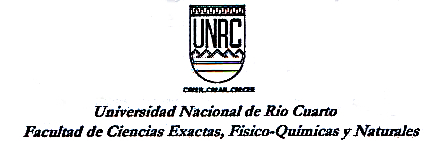
\includegraphics[scale=.4]{membrete.jpg}}]{\fancyplain{}{\vspace{-1cm}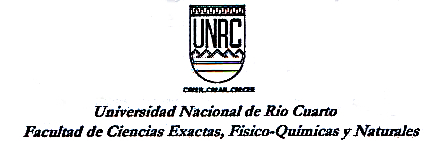
\includegraphics[scale=.4]{membrete.jpg}}}

\cfoot{}













\begin{document}

\title{PLAN DE ESTUDIOS DE LA CARRERA LICENCIATURA EN MATEMÁTICA}
\author{Plan 2022- Versión 0}
\date{}
 \maketitle

 \newpage



\tableofcontents

\newpage


\section{Identificación del proyecto}  

Plan de Estudios de la 
Carrera de Licenciatura en Matemática, de la Facultad de Ciencias Exactas, 
Físico - Químicas y Naturales, de la Universidad Nacional de Río Cuarto. Que reemplaza el Plan de Estudio de la Licenciatrura en Matemática aprobado por resolución del Consejo Directivo Nº 156/08, 
ratificada por resolución del Consejo Superior Nº 212/08.
% Resolución del Consejo Directivo Nº 258 /07, ratificada 
%por Resolución del Consejo Superior Nº 289/07. Registro y toma de conocimiento 
%por parte de la Dirección Nacional de Gestión Universitaria informado por nota 
%Nº 544/08. Introducción de modificaciones, que generaron la versión 1 del Plan 
%de Estudios, aprobadas por 

\section{Responsables del proyecto}

\subsection{Unidad académica responsable de la elaboración del proyecto}

Comisión Curricular Permanente de la carrera Licenciatura en Matemática, dependiente de 
la Facultad de Ciencias Exactas Físico-Químicas y Naturales.

\subsection{Unidad académica responsable de la implementación del proyecto}

Facultad de Ciencias Exactas Físico-Químicas y Naturales.



\section{Fundamentación}

\subsection{Razones que justifican la creación y o los cambios curriculares del proyecto de formación  y que justifican su realización}

A continuación se enumeran normativas que modificaron las existentes al momento de crear la versión anterior del plan de estudios como así también instancias de intercambio institucional que delinearon nuevos paradigmas en la elaboración de planes de estudios e introdujeron nuevas variables a tener en cuenta.
\begin{enumerate}
 \item Que por Resolución CS-UNRC 297/2017 se aprobó el documento ``Hacia   un   currículo contextualizado, flexible e integrado. Lineamientos para la orientación de la innovación  curricular'' que define dimensiones que la Universidad considera importantes a la hora de elaborar planes de estudios, en particular dimensiones epistemólogico-metodológicas, de contextualización, organización, de flexibilidad e integración curricular. 

 \item Que por Resolución CS-UNRC 298/2017 se implementa el Proyecto de Innovación e Investigación para el Mejoramiento Estratégico Institucional (PIIMEI). Como parte de este Proyecto, la Comisión Curricular Permanente de la Licenciatura en Matemática junto con docentes y alumnos de la carrera emprendió una investigación del currículo de la carrera.  Parte de las conclusiones obtenidas fueron plasmandas en un Informe ``Actividades de Investigación Evaluativa
Licenciatura en Matemática'' el cual fue evaluado por expertos en curriculo universitario, los cuales sugierieron acciones a seguir.
\item Que por Resolución CS-UNRC 510/2017 se actualizó el Plan Estratégico Institucional (PEI 2017-2023) el cual se constituye como documento orgánico con miras al desarrollo integral de la universidad, con emplazamiento geográfico y social. Los lineamientos del PEI de la UNRC representan la plataforma desde donde avanzar en la proyección de políticas institucionales de la Universidad en su conjunto y para nuestra Facultad en particular, que atienden necesidades actuales y proponen caminos de actuación a futuro.
\item Que por Resolución CD-FCEFQyN 410/2019 se aprueba el Plan Estratégico de la Facultad de Ciencias Exactas Físico-Químicas y Naturales (PEExa 2019-2023). En particular, en el Capítulo III, Sección 1 define objetivos de la institución para la enseñanza de grado.   

 \item Que por Resolución CS-UNRC 008/2021 se establecen los conceptos, normas y procedimientos que regulan los procesos de elaboración, presentación, formalización, aprobación, seguimiento, evaluación y tramitación de reconocimiento de Nuevos Planes de Estudio y de modificaciones que impliquen nuevas versiones de los Planes de Estudio existentes.

\end{enumerate}

\subsection{Razones que determinan la conveniencia de la implementación de proyecto curricular  y que justifican su realización.}

Implementar los lineamientos propuestos por la Facultad dentro del proyecto PIIMEI. Entre ellos se enumeran:

\begin{enumerate}
\item Contextualización del currículo y visión totalizante.
\item Flexibilidad curricular.
\item Organización curricular mixta.
\item Transversalidad de la práctica profesional.
\item Formación en ciclos o trayectos.
\item Práctica docente de manera transversal a todo el plan de estudio.
\item Inconsistencia de la carga horaria de asignaturas existentes.
\item Actualización curricular.
\item Definición con mayor flexibilidad del ciclo de especialización.
\item Incorporación de espacios de formación socio-cultural.

\end{enumerate}

\subsection{Correspondencia con los fines y objetivos de la
Universidad} 

Los fines y objetivos de la Universidad y de la Facultad de Ciencias, Exáctas Físico-Químicas y Naturales están definidos en el Estatuto Universitario y en el Plan Estratégico Institucional (PEI) y en el Plan Estratégico  de la Facultad (PEExa). El plan de estudios de la Licenciatura de Matemática se enmarca dentro de los objetivos y fines declarados en los anteriores documentos, especialmente por las consideraciones en ellos establecidas  que enumeramos debajo. 


\begin{description}
 \item[Estatuto de la UNRC.]   Aprobado por Resolución Ministerio de Educación Nº1723/2011.  Se define que la Universidad es:
\begin{enumerate}

\item ``Productora, distribuidora y difusora de conocimiento socialmente útil y público, es
decir, provisional, histórico, criticable, no dogmático, hipotético, abierto a la
pregunta, al cuestionamiento y al contraste riguroso. Como tal deberá ser reflexiva
y proactiva, capaz de autoevaluarse en forma permanente y, así, comprender y
mejorar sus procesos y sus productos''


\item ``Una institución que busca la excelencia académica al ofrecer a los estudiantes
conocimientos y prácticas de máxima calidad y de significación científica y social''

\item ``Flexible para adaptarse a la diversificación y expansión de la población estudiantil, 
a las nuevas tecnologías, a las formas de comunicación y producción de
conocimiento, a la movilidad de las profesiones, a la evolución de los paradigmas
de la ciencias y a las nuevas condiciones sociales.''

\item ``Innovadora en sus formas de enseñanza, investigación y transferencia educativa y
tecnológica''

\item ``Una institución articulada con el nivel medio, con el subsistema de educación
superior no universitaria, con otras Universidades de la región, del país y del
mundo y con otras organizaciones sociales y por tener la capacidad de dar
respuestas contextualizadas con lo regional''

\end{enumerate}

\item[PEI 2017-2023] Se definen como Ejes Estratégicos prioritarios en la agenda universitaria:
\begin{enumerate}
 \item Inclusión    educativa    con    calidad    para         todos  los  estudiantes  de  la  universidad  pública.
 
 \item  Actualización  y  flexibilidad  del  currículo  en la enseñanza de grado y posgrado.
 
 \item Producción  de  conocimiento  científico,  técnico y artístico con alto nivel y sentido social. 
\end{enumerate}

\item[PEExa 2019-2023] Define como objetivos de la enseñanza de grado:
\begin{enumerate}
 \item  La actualización curricular.
 \item Sostenimiento y fortalecimiento de la formación integral.
\item Orientación de los procesos de enseñanza y de aprendizaje hacia el
conocimiento de la realidad local, nacional e internacional.
\item Fortalecimiento de modalidades de enseñanza con TICs.
\item Mejoramiento de las prácticas y formación docente.

\end{enumerate}

\end{description}

Por otra parte los objetivos de este plan de estudios están en correspondencia con:

\begin{description}
\item[Prioridades de Investigación de la UNRC] Definidas en la Resolución CS-UNRC 302/2018. 
En ella se consignan las áreas y temas de interés, en particular las área 8 de Matemática y Computación.
\item[Líneas curriculares para la UNRC] Descriptas en las Resoluciones CS-UNRC 297/2017 y 008/2021.
\end{description}




\subsection{Antecedentes}

\subsubsection{Breve reseña del origen y trayectoria de la carrera, considerando los ámbitos nacional, regional e institucional.}

Es dificil rastrear los orígines de la carrera de Licenciatura en Matemática en Argentina. La enseñanza de esta ciencia en territorio argentino se remonta a la  época colonial. Instaurado el primer gobierno patrio, como es sabido, Manuel Belgrano fue un impulsor del estudio de las ciencias. Citando a Edgardo L. Fernández Stacco
 (ver \cite{stacco2011200})
 : ``Producida la revolución, Manuel Belgrano, vocal de la Junta de Gobierno, hizo
crear una Escuela de Matemáticas que puso bajo la dirección del teniente coronel
catalán Felipe de Sentenach, instalada en el 12 de setiembre de 1810. Tenía como
función formar a los oficiales del ejército.
La enseñanza comprendía: aritmética, geometría plana, trigonometría rectilínea
y geometría práctica. Además los oficiales aspirantes a la ingeniería y artillería debían
cursar: Álgebra inferior y superior con sus aplicaciones a la aritmética y la geometría;
mecánica y en particular, estática; secciones cónicas.''

 Una de las primeras menciones que hemos hallado de una carrera denominada Licenciatura en Matemática es en  \cite{ortiz2011julio} 
 donde se menciona que en  1926 se creo una Licenciatura y un Doctorado en Matemática y en Física dentro de una Facultad de Ingeniería. ``Aquella carrera incluía cursos avanzados de matemática pura (análisis y geometría superior) y dos cursos regulares de física-matemática en reemplazo del antiguo curso único de física-matemática del último año de los planes anteriores.Todas estas realizaciones son claramente indicativas de que se comenzaba a prestar mayor  atención a los aspectos teóricos de la ciencia.''

 El estudio de la matemática se ha diseminado por todo el sistema de educación superior Argentino, en la actualidad la carrera de Licenciatura en Matemática se ofrece en las siguientes universidades nacionales: UNRC, UNAB, UNSL, UNC, UNLPam, UNNE, UNICEN, UNL, UNCOMA, UNMDP, UNSJB, UNS, UNSE, UNR y UBA.  
 
 En la UNRC el plan de estudios original data de 1975. Fue elaborado por xxxxxxxx. Posteriormente el plan fue modificado en 1993, 2001 y 2008.  
 
 
 

\begin{description}
 \item[Plan 1975] La carrera de Lic. en Matemática fue una carrera de 5 años de duración que dió inicio en el año 1975 y tuvo su reconocimiento oficial en la Resolución Ministerial N° 1560/80. 

 \includegraphics[scale=.3]{plan1975.png}
 
\item[Plan 1993] Carrera de 5 años

 \includegraphics[scale=.3]{plan1993.png}

\item[Plan 2001] Carrera de 5 años

 \includegraphics[scale=.5]{plan2001.png}


\item[Plan 2008] Carrera de 4 años. Resolución del CD-FCEFQyN Nº 258 /07, ratificada 
por Resolución del CS-UNRC Nº 289/07. Registro y toma de conocimiento 
por parte de la Dirección Nacional de Gestión Universitaria informado por nota 
Nº 544/08. Introducción de modificaciones, que generaron la versión 1 del Plan 
de Estudios, aprobadas por resolución del CD-FCEFQyN Nº 156/08, 
ratificada por resolución del CS-UNRC Nº 212/08.  Nueva introducción de modificaciones, que generaron la versión 2 aprobada por Resolución del CD-FCEFQyN N° 340/17, por la cual se aprueba el Texto Ordenado del Plan de Estudios 2008, Versión 2, de la Carrera de "Licenciatura en Matemática", según consta en el Anexo 1 de la citada Resolución, obrante a fojas 180/216 del Expediente N° 88664.  Resolución del CS-UNRC N° 443/17, por la cual se ratifica la Resolución  CD-FCEFQyN N° 340/17.  La versión 2 del Plan 2008 aún no se encuentra vigente,

 \includegraphics[scale=.75]{plan2008.png}

\end{description}




\subsubsection{Actividades de docencia, investigación o extensión realizadas por Universidad vinculadas  al proyecto.}

\begin{description}
 \item[Docencia] Como se mencionó hay una larga trayectoria  de nuestra Facultad en el dictado de carreras de grado y posgrado  vinculadas con la matemática, particularmente la Licenciatura en Matemática, el Profesorado en Matemática, Maestría en Matemática Aplicada y Especialidad en Didáctica de la Matemática. Además de estos antecedentes, merece mencionarse que diversas carreras de nuestra y de otras facultades requieren el dictado de materias vinculadas con la matemática y por tanto es necesario la formación de docentes altamente calificados en esta disciplina. Nuestros egresados forman parte de los departamentos de matemática de otras facultades de nuestra universidad.
 
 \item[Investigación] Dentro del departamento de matemática de la FCEFQyN se ejecutan regularmente  proyectos financiados tanto por SECyT-UNRC como por organismos de financiamiento nacionales (ANPCyT-CONICET). La modelización matemática y la ciencia de datos proveen una metodología esencial a otras áreas del saber, ingenierías, física, biología, geología, economía, etc. Profesionales egresados de nuestro departamento ejecutan tareas de investigación en las áreas mencionadas en nuestra universidad y en otras instituciones.
 
 
\end{description}






\subsubsection{Experiencias similares realizadas a nivel nacional o internacional que hubieran sido tenidas en cuenta.}

En la elaboración de este plan de estudios se tuvieran en cuenta las siguientes experiencias y antecedentes.
\begin{description}
 \item[Unión Matemática Argentina]  La asociación que agrupa a los matemáticos del país ha convocado a matemáticos de reconicida trayectoria a nivel internacional quienes elaboraron un documento (ver \cite{uma}) 
 dando cuenta de sugerencias curriculares para la carrera de Licenciatura en Matemática.
 
 \item[Foro UMA-CUCEN] En el marco de las reuniones periódicas del Consejo Universitario Ciencias Exactas y Naturales (CUCEN) se realizó durante los años 2017-2018 un foro donde se debatieron ciclos de formación con el propósito de favorecer la movilidad de los estudiantes entre carreras de Licenciatura en Matemática del país. Nuestra carrera participó activamente de este foro. Es de destacar que fruto de esta participación, y como parte del proyecto PIIMEI, se hizo una comparativa entre los distintos planes, más específicamente se definieron distintas nudos conceptuales y se identificaron las carreras de Licenciatura en Matemática de Argentina que trabajan dichos nudos. \textcolor{red}{NOMBRAR INFROME REALIZADO PIIMEI}

\item[Sistema Nacional de Reconocimiento Académico (SNRA)] Fue creado por la Resolución Ministerial N° 1870/16. Es un sistema voluntario de acuerdos entre instituciones de Educación Superior de la Argentina, que permite el reconocimiento de trayectos formativos (tramos curriculares, ciclos, prácticas, asignaturas, materias u otras experiencias formativas) para que los estudiantes transiten por el sistema aprovechando toda su diversidad y profundizando la experiencia de formación.

En el marco del SNRA el Ministerio de Educación convocó a especialistas de todo el sistema de educación superior, incluído doncentes de nuestra Licenciatura en Matemática,  para que definan trayectos formativos con el propósito de facilitar la movilidad estudiantil dentro del sistema de ecucación superior nacional. 

Fruto de la participación antes aludida nuestra universidad suscribió convenios de reconocimiento de trayectos académicos dentro del área matemática. Este plan de estudio refleja los acuerdos expresados dentro de estos convenios.

\item[Proyecto Tuning] Tuning es una red de comunidades de aprendizaje de alcance internacional, integrada por académicos y estudiantes interconectados, que reflexiona, debate, elabora instrumentos
y comparte resultados. Siguiendo a \cite{paniagua2013educacion},
 ``Tuning es una metodología con pasos bien diseñados, y una perspectiva dinámica que permite la adaptación a los diferentes contextos. La metodología tiene un objetivo claro: construir titulaciones compatibles, comparables, relevantes para la sociedad y con niveles
de calidad y excelencia, preservando la valiosa diversidad que viene de las
tradiciones de cada uno de los países.'' 

Para el diseño de la presente propuesta curricular se tuvo en consideración el documento \cite{paniagua2013educacion} 
que estudia perfiles del egresado y escenarios de futuro para el Área de Matemática y la profesión y estrategias de enseñanza, aprendizaje y evaluación de las competencias propias de los profesionales del área. 

\item[Competencias matemáticas para la industria] 
Es una preocupación permanente en el diseño del plan de estudios de la Licenciatura en Matemática, tanto en esta institución como otras, la inserción del egresado en ámbitos no académicos. Generalmente se refiere a estos ámbitos como la ``industria'' en la bibliografía, aunque se comtempla que estos incuyen organismos públicos, empresas informáticas, etc. Diversas organizaciones se han encargado de identificar aquellas competencias que son requeridas en industrias a profesionales y que pueden ser provistas por egresados del área de las matemáticas y han propuesto estrategias pedagógicas para la consecución de estas competencias. Hemos estudiado los siguientes antecedentes en esta materia.

La Society for Industrial and Applied Mathematics (SIAM)  es una asociación académica dedicada al uso de las matemáticas en la industria que tiene conexiones con la Asociación Argentina de Matemática Aplicada Computacional e Industrial. La SIAM publicó varios documentos sobre la problemática del matemático en la industria, en particular \cite{society1996siam,society2012siam}.


 La Comisión Internacional de Instrucción Matemática (ICMI) es una comisión de la Unión Internacional de Matemáticas (IMU) y es una organización de actuación internacional centrada en la educación matemática. La ICMI publicó las Educational Interfaces between Mathematics and Industry (ver \cite{damlamian2013educational}) entre otros materiales dirigidos a la temática en cuestión.
\end{description}



\subsubsection{Población destinataria}

La población destinataria de la carrera es la definida por la Resolución CS-UNRC 120/2017 que aprobó el ``Régimen  de estudiantes y de enseñanza de pregrado y grado de la UNRC''. En el punto 2 del Anexo I de la mencionada normativa se establecen las condiciones para que un estudiante ingrese a una carrera de grado dentro del ámbito de la UNRC.




\subsubsection{Rasgos y características de la población estudiantil que atiende: tener en cuenta los destinatarios reales y potenciales de la formación, considerando las condiciones y cualidades sociales, culturales y económicas que la caracterizan en general y según los grupos de procedencia: diversidades culturales, mayores de 25 años sin título secundario, culturas juveniles vigentes y emergentes, personas en situación de discapacidad, adultos mayores, estudiantes de pueblos originarios, de diferentes lugares del país y extranjeros, entre otros.}

\textcolor{red}{Cómo caracterizaríamos nuestros estudiantes? VER ARCHIVO COMPARTIDO POR MARCELO}

\section{Objetivos del proyecto}
\subsection{Objetivos generales}

Formar egresados con un alto conocimiento técnico en una
disciplina considerada estratégica en el desarrollo futuro del
país (ver por ejemplo la convocatoria a subsidios PAV efectuada
por la SECYT de la Nación \cite{pav2003}).


Capacitar para el uso de las herramientas matemáticas en la
resolución de problemas científicos y/o tecnológicos.

Brindar  al egresado  conocimientos sólidos en la disciplina
matemática que le permita acceder a carreras de posgrado y/o
participar en grupos de trabajo interdisciplinario.

Formar profesionales capacitados en la metodología de la investigación matemática y capaces de plantear y resolver problemas en esa área del saber.

\subsection{Objetivos específicos}


\begin{enumerate}

\hyphenation{a-sig-na-tu-ras}
    \item Profundizar la  formación interdisciplinaria del
    egresado.
    \item Incorporar nuevos  recursos
    informáticos en las distintas asignaturas.
    \item Fortalecer la integración curricular con el Profesorado
    en Matemática preservando las identidades de cada carrera.
    \item Promover un cambio paulatino en las metodologías de
    enseñanza de la matemática en nuestro departamento.

    \item Alentar al estudiante para que tome contacto con problemas de
    investigación en distintos momentos de la carrera culminando
    en un ciclo de especialización con una marcada formación en
    investigación.

    \item Brindar al alumno la posibilidad de integrarse tempranamente
    a las temáticas de su preferencia.

\end{enumerate}





\section{Características de la carrera}


\subsection{Nivel} Carrera de grado.

\subsection{Acreditación} Licenciado en Matemática.

\subsection{Alcance del título} Esta carrera habilita para:
\hyphenation{de-sa-rro-llo}
    \begin{enumerate}

        \item Participar en equipos interdisciplinarios realizando
         tareas de asesoramiento en temas específicos.
        \item  Realizar actividades de investigación en proyectos de matemática
        pura o aplicada.
       \item Intervenir  como peritos matemáticos en instituciones tales como
       empresas que realicen desarrollos tecnológicos, bancos,
       compañías de seguro, etc.
        \item Acceder a carreras de posgrado.
         \item Participar de los equipos docentes dirigidos a la
         enseñanza de la matemática en los niveles superiores de enseñanza.
    \end{enumerate}

\subsection{Actividades profesionales reservadas al título (Incumbencias)}
    
\subsection{Perfil del Título}
\textcolor{blue}{asesorarse}


\subsubsection{Conocimientos que constituyen el fundamento teórico-metodológico de su accionar profesional o académico.}

Se aspira a que el Lic. en Matemática adquiera un conocimiento sólido en las siguientes  áreas de
 la matemática: Análisis Matemático, Funciones de una Variable Compleja,   Teoría de la Medida, Probabilidades y Estadística, Ciencia de Datos, Geometría Diferencial, Álgebra Lineal, Estructuras Algebracicas, Ecuaciones Diferenciales ordinarias y parciales, Cálculo Numérico, Análisis Funcional y Modelización Matemática.

 Se aspira además a que el estudiante logre una formación complementaria en un área de su elección dentro de la oferta de que disponga como parte de su ciclo de especialización.
 
\subsubsection{Capacidades y habilidades requeridas para la realización de las actividades que le incumben.}

\begin{enumerate}

\item {Responsabilidad social y compromiso
ciudadano.} 



\item {Capacidad de aprender, actualizarse y trabajar de manera autónoma.} 
 


\item {Capacidad crítica y autocrítica.} 
 

\item {Valoración y respeto por la diversidad
y multiculturalidad.} 
 




\item {Dominio de los conceptos básicos
de la matemática superior.} 
 

\item {Capacidad para construir y desarrollar
argumentaciones lógicas con una
identificación clara de hipótesis y conclusiones.} 
 
\item {Capacidad de abstracción (extraer de una situación los rasgos más relevantes).} 
 


\item {Capacidad para formular problemas
en lenguaje matemático.} 
 

  


\item {Capacidad para iniciar investigaciones
matemáticas bajo orientación de experto.} 
 


\item {Capacidad para formular problemas
de optimización, tomar decisiones e interpretar
las soluciones en contextos originales
de los problemas.} 
 


\item {Capacidad para contribuir en la
construcción de modelos matemáticos a
partir de situaciones reales.} 
 


\item {Capacidad para utilizar las herramientas
computacionales de cálculo numérico
y simbólico para plantear y resolver
problemas.} 
 


\item {Capacidad para extraer información
cualitativa de datos cuantitativos.} 
 


\item {Capacidad para expresarse correctamente
utilizando el lenguaje de la
matemática.} 
 


\item {Capacidad para comunicarse
con otros profesionales no matemáticos.} 

 

\item {Capacidad para actuar en contextos educativos y planificar actividades de enseñanza} 
 


\item {Conocimiento del inglés para
leer, escribir y exponer documentos en
inglés, así como comunicarse con otros
especialistas.} 

 


\item {Capacidad para trabajar en equipos
interdisciplinarios.} 

\end{enumerate}


\subsection{Requisitos de ingreso}



Los fijados por el ``Régimen  de estudiantes y de enseñanza de pregrado y grado de la UNRC'', ver  el punto 2 del Anexo I de la Res. CS. 120/2017. 



\subsection{Organización del Plan de Estudios}
\begin{colortext}{blue}
\subsubsection{Ciclos, Trayectos  y Áreas} El Plan de Estudios se desarrollará en tres ciclos:
un ciclo básico común con el profesorado, un ciclo superior y un
ciclo de especialización.

\paragraph{Ciclo Básico} El ciclo básico incluye 12 asignaturas.

\setlength\arrayrulewidth{1pt}
\begin{center}
\begin{tabular}{|l|r|r|r|}\hline
  \rowcolor[gray]{.9}
  \emph{Asignaturas del ciclo básico} & Código  & \emph{Horas semanales} &  \emph{Horas totales}
  \\\hline
  Cálculo I                          &   1921   &           8 hs  &   120 hs         \\ \hline
  Matemática Discreta       	     &   1925   &           8 hs  &   120 hs         \\ \hline
  Geometría I               	     &   1935   &           6 hs  &    90 hs         \\ \hline
  Cálculo II                         &   1928   &           8 hs  &   120 hs         \\ \hline
  Álgebra Lineal I                   &   1933   &           8 hs  &   120 hs         \\ \hline
  Taller de informática              &   1927   &           6 hs  &    90 hs         \\ \hline
  Cálculo III                        &   1929   &           8 hs  &   120 hs         \\ \hline
  Probabilidades                     &   1987   &           8 hs  &   120 hs         \\ \hline
  Estructuras Algebraicas            &   1993   &           8 hs  &   120 hs         \\ \hline
  Taller de Resolución de Problemas  &   1994   &           4 hs  &    60 hs         \\ \hline
  Estadística                        &   1991   &           6 hs  &    90 hs         \\ \hline
  Física                             &   1930   &           6 hs  &    90 hs         \\ \hline
  \emph{Total de horas ciclo básico }& \multicolumn{3}{r|}{\emph{1260hs}}            \\ \hline
\end{tabular}
\end{center}


\paragraph{Ciclo Superior} Consta de 10 materias
obligatorias.

\begin{center}
\begin{tabular}{|l|r|r|r|}\hline
  \rowcolor[gray]{.9}
\emph{Asignaturas del ciclo superior  }  & Código &\emph{Horas semanales} &  \emph{Horas totales}\\ \hline
Inglés  (Anual)                            & 1976   &           4 hs        &     120 hs           \\ \hline
Estudio de la Realidad Nacional          & 6235   &           2 hs        &      30 hs           \\ \hline
Cálculo Numérico  Computacional          & 2030   &           8 hs        &     120 hs           \\ \hline
Topología                                & 1917   &           9 hs        &     135 hs           \\ \hline
Álgebra Lineal Aplicada                  & 2261   &           7 hs        &     105 hs           \\ \hline
Variable Compleja y Análisis de Fourier  & 2262   &           9 hs        &     135 hs           \\ \hline
Medida e Integración                     & 2263   &           8 hs        &     120 hs           \\ \hline
Ecuaciones Diferenciales                 & 1913   &           8 hs        &     120 hs           \\ \hline
Geometría Diferencial                    & 1915   &           8 hs        &     120 hs           \\ \hline
Modelos Matemáticos                      & 2265   &           6 hs        &      90 hs           \\ \hline
Modelos de regresión y metodos empíricos  & XXXX  &           6 hs 
& 90 hs   \\ \hline
\emph{Total de horas ciclo superior }    &\multicolumn{3}{r|}{\emph{1095 hs}}                    \\ \hline
\end{tabular}
\end{center}



\paragraph{Ciclo de Especialización} Dirigido a introducir al alumno
en el estudio de una rama específica de la matemática a su
elección. Incluye un \emph{seminario}
 destinado a orientar al alumno en su decisión.  Además consta de asignaturas
\emph{optativas}, en un mínimo de dos y un máximo de cuatro que
reúnan en total una suma de 270 horas y un \emph{trabajo final} de
150 horas. Las optativas deberán ser realizadas bajo la dirección
de un docente tutor del Departamento de Matemática a elección del
alumno y con anuencia del Consejo Departamental y de la Comisión
Curricular de la Licenciatura en Matemática. El tutor orientará al
estudiante en la selección de las optativas, que podrán ser
realizadas en este Departamento o en otro Departamento de la
Universidad. El trabajo final deberá ser realizado bajo la
dirección del docente tutor de acuerdo a las normativas de la
Facultad de Ciencias Exactas Fco-Qcas y Naturales.


Actualmente el Dpto. brinda las siguientes orientaciones.




\begin{enumerate}
\item[A.] Análisis Matemático,
\item[B.]  Matemática Aplicada,
\item[C.] Didáctica de la Matemática,
\item[D.] Estadística.
\item[E.] Geometría, Álgebra y Grupos de Lie.
\end{enumerate}

Propuestas de otras orientaciones serán evaluadas por la C. C.
permanente de la carrera.

\begin{center}
\begin{tabular}{|l|r|r|}\hline
  \rowcolor[gray]{.9}
\emph{Asignaturas del ciclo de especialización  } & Código & \emph{Horas totales}      \\ \hline
Seminario de Especialización                      & 2264   &   45 hs                   \\ \hline
Optativas                                         &        &  270 hs                   \\ \hline
Trabajo Final                                     & 2038   &  150 hs                   \\ \hline
\emph{Total de horas ciclo de especialización}    & \multicolumn{2}{r|}{\emph{465 hs}} \\ \hline
\end{tabular}
\end{center}


\newpage

\end{colortext}

\subsubsection{Listado total de asignaturas}
\fontsize{8pt}{8pt}\selectfont  
\begin{center}
\begin{xtabular}{|l|r|l|r|r|}\hline
\rowcolor[gray]{.9}\multicolumn{5}{|c|}{\textbf{Primer año}}                                                        \\ \hline

\emph{Cuat. }  &\emph{Código}  & \emph{Materia}                              &    hr. sem.       &  hr. Tot.        \\ \hline

I              & 1921          & Cálculo I                                &          8  &   112     \\ \hline
I              & 1925          & Matemática Discreta                      &          8  &   112       \\ \hline
I              & 1935          & Geometría I                              &          6  &    84       \\ \hline
\multicolumn{3}{|l|}{\textbf{Total de Horas cuatrimestre I}}              &\textbf{22 } &\textbf{308 }\\ \hline
II             & 1928          & Cálculo II                               &          8  &   112       \\ \hline
II             & 1933          & Álgebra Lineal I                         &          8  &   112       \\ \hline
II             & 1927          & Taller de informática                    &          6  &    84       \\ \hline
\multicolumn{3}{|l|}{\textbf{Total de Horas cuatrimestre II}}             &\textbf{22 } &\textbf{308 }\\ \hline
 
\rowcolor[gray]{.9}
\multicolumn{5}{|c|}{\textbf{Segundo año}}                                                                \\ \hline
III            & 1929          & Cálculo III                              &          8  &   112      \\ \hline
III            & 2030          & Cálculo Numérico  Computacional          &          8  &   112    \\ \hline
III            & 1976          & Inglés (Anual)                           &          4  &    56     \\ \hline
\multicolumn{3}{|l|}{\textbf{Total de Horas cuatrimestre III}}            & \textbf{20 }&\textbf{280 }\\ \hline
IV             & 1987          & Probabilidades                           &          8  &   112      \\ \hline
IV             & 1993          & Estructuras Algebraicas                  &          8  &   112      \\ \hline
IV    &  1976 & Inglés (Anual) & 4  & 56 \\ \hline
\multicolumn{3}{|l|}{\textbf{Total de Horas cuatrimestre IV}}             &\textbf{20 } &\textbf{280 }\\ \hline

\rowcolor[gray]{.9}\multicolumn{5}{|c|}{\textbf{Tercer año}}                                                        \\ \hline
V              & 1991          & Estadística                                &           6         &         84         \\ \hline
V              & XXXX          & Fundamentos de Análisis           &            8        &             112     \\ \hline
V             & 2261          & Álgebra Lineal Aplicada                  &          8  &   112       \\ \hline

\multicolumn{3}{|l|}{\textbf{Total de Horas cuatrimestre V}}                &\textbf{22}           &\textbf{308}         \\ \hline
VI             & 1930          & Física                                     &            6        &           84       \\ \hline
VI             & 2262          & Variable Compleja                          &             8       &         112         \\ \hline
VI             & 6235          & Estudio de la Realidad Nacional *          &               2     &         28         \\ \hline
VI            & 1917          & Topología                                   &              8      &        112          \\ \hline
\multicolumn{3}{|l|}{\textbf{Total de Horas cuatrimestre VI} }              &\textbf{24}           &\textbf{336}         \\ \hline
  
\rowcolor[gray]{.9}\multicolumn{5}{|c|}{\textbf{Cuarto año}}                                                        \\ \hline
VII           & 2263          & Medida e Integración                       &             8       &            112      \\ \hline

VII            & 1913          & Ecuaciones Diferenciales                   &           8         &        112          \\ \hline
\multicolumn{3}{|l|}{\textbf{Total de Horas cuatrimestre VII}}              & \textbf{24}          &\textbf{336}         \\ \hline
VIII             & 1915          & Geometría Diferencial                      &              8     &        112          \\ \hline
VIII           & xxx           & Modelos de regresión y metodos empíricos                  &              6      &         84         \\ \hline

% VIII           & 2265          & Modelos Matemáticos                        &               6     &       84           \\ \hline

VIII          & 2212           & Introducción a las Ecuaciones en Derivadas Parciales & 8  & 112  \\ \hline

\multicolumn{3}{|l|}{\textbf{Total de Horas cuatrimestre VIII}}             & \textbf{20}          &\textbf{280}         \\ \hline

\rowcolor[gray]{.9}\multicolumn{5}{|c|}{\textbf{Quinto año}}                                                        \\ \hline
IX            &  1916         &  Análisis Funcional               &           8         &            112      \\ \hline
IX           &               & Optativa I                                &            10        &         140         \\ \hline
\multicolumn{3}{|l|}{\textbf{Total de Horas cuatrimestre VII}}              & \textbf{}          &\textbf{}         \\ \hline
X           &               & Optativa II                                &           10         &          140        \\ \hline
X           & 2265          & Trabajo Final                              &                    &                  \\ \hline
X           &           & Electiva                             &                    &                  \\ \hline

\multicolumn{3}{|l|}{\textbf{Total de Horas cuatrimestre VIII}}             & \textbf{}          &\textbf{}         \\ \hline
\multicolumn{4}{|l|}{\textbf{Total de Horas del Plan de estudios}}                               &\textbf{}         \\ \hline






\end{xtabular}
\end{center}
\normalsize



\subsubsection{Contenidos y metodología}
\paragraph{Contenidos}
\subparagraph{Ciclo Básico}

\begin{enumerate}

\item \textbf{Cálculo I (1921):} Números Reales. Funciones
trascendentes. Operaciones con funciones. Límite. Continuidad.
Derivadas. Aplicaciones de la Derivada: máximos, mínimos, trazado
de curvas. Teorema del valor medio: Aplicaciones.

Bibliografía Principal: \cite{PeterD.Lax631}.

Bibliografía Consulta: \cite{MichaelSpivak649}

Bibliografía orientada por la historia: \cite{ErnstHairer633,DavidApplebaum639,OttoToeplitz642,DavidBressoud643,DavidM.Bressoud651,DavidM.Bressoud688}.


 
\item \textbf{Matemática discreta (1925):} Introducción a la lógica. Números
naturales. Principio de inducción. Introducción a la combinatoria.
Números enteros: Divi\-sibilidad, Teorema fundamental de la
Aritmética, Congruencia,  Ecuaciones Diofánticas, Teorema de
Fermat y Euler. Relaciones y funciones: funciones inyectivas,
suprayectivas, relaciones de orden y de equivalencia.

Bibliografía Principal: \cite{gentile, grimaldi}.




\item \textbf{Geometría I (1935):} Triángulos: medianas, mediatrices, centroides. Inscriptos y
circunscriptos. Ortocentro. Polígonos: simetrías. Isometrías del
plano euclídeo. Geometría afín: ecuaciones de rectas  en
el plano y de rectas y planos en el espacio. Espacios vectoriales generales.
Transformaciones lineales: rotaciones, reflexiones, simetrías.
Cónicas y cuádricas.
Bibliografía Principal: \cite{AllanBerele41,RogerFenn248,RobinHartshorne131,AlfredS.Posamentier49}.

Bibliografía de Consulta: \cite{O.Bottema149,CharlesStanleyOgilvy129,AllanBerele41,GerardA.Venema145,H.S.M.Coxeter226,H.S.M.Coxeter35,MatthewHarvey261,RogerA.Johnson42,coxeter,GJE,villamayor}.




\item \textbf{Cálculo II (1928):}   Integral definida de una variable real: áreas, volúmenes,
longitudes, etc. Métodos de integración, integrales impropias.
Sucesiones y series numéricas. Series de potencias. Series de
Taylor. Introducción a las  ecuaciones diferenciales de primer
orden.


Bibliografía Principal: \cite{PeterD.Lax631,GeorgeFinlaySimmons487}.

Bibliografía Consulta: \cite{MichaelSpivak649,ErnstHairer633,DavidApplebaum639,OttoToeplitz642,DavidBressoud643,DavidM.Bressoud651,DavidM.Bressoud688}.





\item \textbf{Taller de Informática (1927).} Noción de algoritmo. Su formulación en pseudocódigos. Estructuras de datos y de control. Implementación
en lenguaje computacional.

Bibliografía sugerida: \cite{Seroul:2000,Rose:2015}.




\item \textbf{Álgebra Lineal I (1933):} Espacios vectoriales. Transformaciones
lineales y matrices. Teorema de la dimensión. Rango de una matriz.
Espacio dual. Espacio euclídeo. Bases ortonormales. Polinomios.
Autovalores y autovectores. Dia\-gonalización.

Bibliografía sugerida: \cite{hoffman, strang}.


\item \textbf{Cálculo III (1929):} Funciones vectoriales. Derivadas. Longitud de
arco. Funciones de varias variables. Derivadas parciales. Regla de
la cadena. Derivadas direccionales. Extremos y extremos
condicionales. Integración múltiple. Aná\-lisis vectorial.
Integrales de línea y de superficie. Teoremas de Green, Gauss y
Stokes.

Bibliografía sugerida: \cite{ marsdentromba,MarianoGiaquinta641,ErnstHairer633,PeterD.Lax632}.




\item\textbf{Inglés (1976):} Inglés nivel básico: Verbos \emph{to be}, \emph{to
have}. Uso de \emph{some} y \emph{any}. El presente simple. El
pasado simple. Uso de little, \emph{few, much, many, each, either,
every, both}. La voz pasiva. La forma \emph{ing}. El infinitivo.
Expresiones de comparación. Formas superlativas. Sentencias
condicionales. Futuro simple.  Análisis de textos relacionados con la
ciencia matemática; enfatizando el reconocimiento de: elementos no
ling\"{u}ísticos, elementos ling\"{u}ísticos ( nivel: léxico,
sintético, morfológico y semántico) y funciones del lenguaje
(descripción, definición, clasificación, etc.).



\item \textbf{Probabilidades (1987):} Espacios de probabilidad.  Probabilidad
condicional e independencia.  Variables aleatorias y sus distribuciones.  Vectores aleatorios y transformaciones.  Dependencia y distribuciones condicionales. Función generatriz de momentos y sus aplicaciones. Convergencia de variables aleatorias. Ley débil y ley fuerte de
los grandes números. Teorema Central del Límite. 

Bibliografía sugerida: \cite{berts, parzen, ross, grimmet}. 

\item \textbf{Estructuras Algebraicas  (1993):} Grupos. Grupos cíclicos y
simétrico. Acción de un grupo en un conjunto. Teoremas de Sylow.
Anillo. Dominios Euclidianos, Principales y de Factorización
única. Módulo. Módulos: Finitamente Generados, Libres.
Divisibilidad.

Bibliografía sugerida: \cite{ gentile,herstein, lang}.



\item\textbf{Álgebra Lineal Aplicada (2261):}  Normas matriciales.
Método de Gram-Schmidt. Descomposición QR.
Matrices unitarias y ortogonales. Reducción ortogonal.
Descomposición SVD. Diagonalización. Matrices normales y simétricas. Matrices
definidas positivas. Matrices nilpotentes y formas de Jordan.

 Bibliografía sugerida: \cite{golub,hoffman,meyer, strang}


 \item \textbf{Estadística (1991):} Estadística Descriptiva. Distribuciones de muestreo. Estimación Puntual. Intervalos y Regiones de Confianza. Pruebas de Hipótesis. Pruebas de $\chi$-Cuadrado. Modelos de regresión lineal. Métodos empíricos. 

Bibliografía sugerida: \cite{wasserman, devore, witten, boente, mosche}
 
\item \textbf{Fundamentos de análisis:} Cardinalidad. Espacios métricos. Completitud. Conexión. Compacidad. Convergencia uniforme. $M$-test Weiertrass. Series de potencias y de Fourier. Convergencia uniforme y su relación con la continuidad, la  derivada y la  integral. Teorema punto fijo de Banach. Aplicación: Teorema de Existencia y Unicidad de soluciones ecuaciones diferenciales ordinarias.  
Bibliografía sugerida: \cite{RogerGodement658,StephenAbbott134,Simmons671,MichealOSearcoid674,SatishShirali675,VictorBryant676,J.Dieudonne678,WalterRudin681,NikolaosKatzourakis684,VilmosKomornik685,VicenteMontesinos686}











\item\textbf{Física (1930):} Mecánica. Dinámica de una partícula. Leyes
de Newton. Concepto de masa. Energía cinética y potencial. Fuerzas
de vínculo. Fuerza centrípeta. Fuerzas de rozamiento. Ley de
gravitación universal. Ecuaciones de movimiento. Momentos. Fuerzas
angulares. Trabajo y energía. Campos conservativos.
Potencia. Cinemática y  dinámica del cuerpo rígido. Momento de
inercia. Teorema de Steiner. Sistemas no inerciales. Teoría de
errores.

Bibliografía sugerida: \cite{roederer, sears}.


\item\textbf{Variable Compleja:}
Funciones analíticas. Desarro\-llos en serie de potencias. Fórmula
y teorema de Cauchy. Singularidades. Series de Laurent. Cálculo de
residuos. Mapeo conforme. Aplicaciones a problemas de Dirichlet y Poisson.

Bibliografía sugerida: \cite{ahlfors, churchill,conway}



\item\textbf{Estudio de la Realidad Nacional (6235):} Derechos y garantías constitucionales. Protección de los derechos humanos. Instituciones políticas.
El estado. Organización jurídica-política de la Repúiblica Argentina. Partidos políticos y sistemas de
mediación, representación y participación. La democracia. La sociedad. Estructura. Problemas. El
sistema económico. La educación. Universidad. Ética profesional.
\textcolor{green}{Preguntar si es posible reemplazar este espacio por participaciones en organismos colegiados, centros de estudiantes, etc}


\item\textbf{Geometría Diferencial (1915):} Geometría de curvas y superficies.
 Geometría Riemanniana
intrínseca. El Teorema de Gauss Bonnet. Variedades diferenciales $k$-dimensionales.
Bibliografía Sugerida: \cite{docarmo,morgan,oneill}
\hyphenation{de-fi-ni-das}




\item\textbf{Cálculo Numérico Computacional (2030):} Sistemas de Numeración.
Teoría de errores. Solución de ecuaciones lineales y no-lineales.
Aproximación e Interpolación de funciones. Integración numérica.
Producto escalar discreto y continuo. Polinomios ortogonales y
cuadrados mínimos. Implementación de los algoritmos numéricos en
un lenguaje computacional.

Bibliografía sugerida: \cite{burden, cheney}.



\item\textbf{Topología (1917):}  Espacios topológicos. Funciones continuas. Subespacios, espacios producto
y cociente. Axiomas de separación. Metrización.
Conjuntos compactos y conexos. Espacios de funciones Teorema de Arzela-Ascoli. Teorema de Weiertrass. 
 Topología Algebraica. Homotopía.

Bibliografía Sugerida: \cite{dugundji, kelley,
munkres, morris1989topology,  JohnMcCleary84,StefanWaldmann87,JohnB.Conway251, RobertAConover507}.

\item\textbf{Ecuaciones Diferenciales (1913):} Ecuaciones de primer
orden. Ecuaciones lineales de orden superior. Método de Frobenius. Sistemas lineales. Problemas de Sturm-Liouville.

Bibliografía Sugerida: \cite{ GeorgeFinlaySimmons487,WilliamE.Boyce496, MorrisW.Hirsch540,JorgeSotomayor513,BarbaraD.MacCluer515,RichardS.Palais519,GarrettBirkhoff526}


\item\textbf{Introducción a las Ecuaciones en Derivadas Parciales (2212):}  Ecuaciones de la Física-Matemática. Ecuaciones de primer orden. Método de características. Ecuación de Laplace. Teorema del valor medio. Teorema del máximo. Desigualdad de Harnack. Ecuación del Calor. Nucleo del calor. Operadores de convolución.  Método de Fourier. Problemas de Sturn-Liouville.  Ecuación de ondas. Método de características. Leyes de conservación. Formula de D'{}Alembert. Medias esféricas. 

Bibliografía sugerida: \cite{LawrenceC.Evans271,WalterCraig494,AlexanderKomech496,JulianFernandezBonder511,DavidBorthwick689,FritzJohn692,SandroSalsa693,AndrasVasy695,YehudaPinchover697,PavelDrabek698, AslakTveito699}.



\item\textbf{Medida e Integración (2263):}  Medida de Lebesgue. Funciones medibles.
Integral de
Lebesgue. Lema de Fatou y Teorema de la Convergencia Mayorada.
Teorema de Fubini. Espacios de Banach y de Hilbert. Espacios
$L^p$. Espacio  $L^2$. Bases ortonormales. Series de Fourier.
Funciones de variación acotadas y absolutamente continuas. 

Bibliografía sugerida: \cite{favazo, loeve, rudin, EliasM.Stein105,TerenceTao123,A.N.Kolmogorov682,DavidM.Bressoud121,wheeden2015measure}.



\item\textbf{Modelos de regresión y metodos empíricos}

 Técnicas de remuestreo. Métodos de regresión en alta dimensión. Ridge, Lasso, Elastic net. Grouped Lasso. Ensambles. Componentes principales para regresión. Selección de Variables. Modelos Aditivos. Métodos basados en Árboles. Árboles para regresión y clasificación. Datos Faltantes. Boosting




\end{enumerate}

\subparagraph{Ciclo de Especialización} Consta de la siguiente
asignatura obligatoria:



\textbf{Seminario de Especialización (2264):} Espacio curricular
destinado a orientar al alumno en torno a su decisión de la línea
a seguir en sus estudios. Para su implementación, cada año el
Consejo Departamental designará un docente encargado de coordinar
 un ciclo de charlas donde  integrantes de cada uno
de los proyectos de investigación del Dpto. y, eventualmente,
invitados externos al Dpto, informarán al estudiante sobre las
distintas líneas de investigación que podría elegir para el ciclo
de especialización. El alumno obtendrá la regularidad con el 80\%
de asistencia y la aprobación con la elaboración de un escrito
relacionado con el tema escogido, para lo cual previamente elegirá
un docente tutor que asesorará la elaboración del escrito y
evaluará el mismo junto al docente coordinador.



\textbf{Plan de especialización:} Es el plan que deberán presentar el alumno con el  docente tutor al Consejo Departamental, con el detalle de las materias optativas que cursará el alumno y un proyecto de Trabajo Final. Es requisito para presentar el mismo tener

\begin{itemize}
\item aprobadas todas las asignaturas de los primeros dos años de la carrera.
\item regularizadas el 70\% de las horas correspondientes a las asignaturas de tercer año.
\item aprobado el \emph{Seminario de especialización}.
\end{itemize}
Habiendo recibido el plan, el Consejo Departamental lo analizará con el asesoramiento de la Comisión Curricular Permanente de la Licenciatura en Matemática, para luego elevarlo a la Secretaría Académica de la Facultad para su aprobación.
\hyphenation{si-guien-tes}

\textbf{Trabajo Final (2038):} El trabajo
final se elaborará a partir de alguna/s de las siguientes
alternativas:
\begin{itemize}
\item un trabajo de investigación realizado por el alumno,
\item un trabajo de síntesis de artículos de investigación publicados en
revistas de reconocido prestigio,
\item una experiencia de aplicación de la matemática en grupos interdisciplinarios
y/o en empresas.
\end{itemize}

El alumno realizará una monografía que a posteriori defenderá
oralmente siguiendo las normas establecidas por la Facultad de Ciencias Exactas, Fís-Qcas y Naturales.



\subsubsection{Transversalidad de contenidos y metodología: explicitación de los contenidos y metodologías transversales en los diferentes campos disciplinares o en espacios interdisciplinares.} \textcolor{green}{Nuevo}

\subsubsection{Correlatividades}
 \textcolor{green}{Hay que cambiar}
\fontsize{9pt}{9pt}\selectfont
\begin{center}
\begin{tabularx}{\textwidth}{|l|l|l|p{3cm}|X|X|X|X|}\hline
\rowcolor[gray]{.9}
\multicolumn{8}{|c|}{Materias Obligatorias}\\ \hline
\rowcolor[gray]{.9}
Año  &    Cuat. & Código   & Asignatura &  \multicolumn{2}{|c|}{Para Cursar}  & \multicolumn{2}{|c|}{Para Rendir}\\ \hline
     &          &          &            & Regular & Aprobada & Regular &Aprobada \\ \hline
I  & 1    & 1921   &    Cálculo I  &--&--&--&-- \\ \hline
I  & 1    & 1925   &  Matemática Discreta&--&--&--&-- \\ \hline
I  & 1   &  1935 &   Geometría I        &--&--&--&-- \\ \hline
I  & 2   &  1928 & Cálculo II            &1921 &-- &--&1921 \\ \hline

I  & 2   &1933    &Algebra Lineal I    &1925 &--&--&1925 \\ \hline

I  & 2   &1927    &Taller de Informática  &1925  &--&--& 1925 \\ \hline

II & 1   &1929    & Cálculo III          & 1933\newline 1928 &1921 \newline 1935&--& 1933\newline 1928  \newline 1935 \\ \hline

II   & 1  &  2030  &Cálculo Numérico Computacional &1928 \newline 1927 &1921 &--&
1928\newline
1927\\ \hline

II & A &   1976 &  Inglés &--&--&--&-- \\ \hline

II & 2 &1987 & Probabilidades  &1928 &-&---&1928\\ \hline

II & 2& 1993 &Estructuras Algebraicas &1933&1925&--& 1933\\ \hline

II & 2 & 2261 & Algebra Lineal Aplicada &--&1933&--&1933 \\ \hline

III & 1 & 1991 & Estadística &1987&--&--&1987 \\ \hline

III &1 & 1930 &Física  &--&1929&--&1929 \newline
\\ \hline

III & 1 & 1917 &Topología &-- &1929&--&1929 \\ \hline

III & 2 &2262 &Variable Compleja y \newline Análisis de Fourier &1917&-&---&1917 \\ \hline

III & 2 &2263 &Medida e Integración &1917&--&--&1917 \\ \hline

III & 2 &1994 &Taller de Resolución de Problemas  &--&1925\newline
1935\newline
1928 &--&1925 \newline
1935\newline
1928\\ \hline

III & 2 & 2264 & Seminario de Especialización &1917\newline
1993&--&--&1917\newline
1993\\ \hline

III & 2 & 6235 & Estudio de la Realidad Nacional &--&--&--&--\\ \hline



IV & 1 & 1913 & Ecuaciones Diferenciales &1917\newline
2261&--&--&1917\newline
2261\\ \hline

IV & 1 & 1915 & Geometría Diferencial & 1917\newline
2261 &--&--& 1917\newline
2261\\ \hline

IV & 2 & 2265 & Modelos Matemáticos &1913&2261\newline
2030&--&1913\newline
2030\\ \hline

IV & 2 & 2038 & Trabajo Final & 2261 &2263\newline 1976 &--& 2261\newline
2263\newline 1976 \\ \hline
\end{tabularx}

\end{center}
\normalfont









\subsubsection{Otros requisitos necesarios para el cumplimiento del Plan de Estudios: señalar los seminarios, trabajos de campo, prácticas profesionales, residencias, idiomas, trabajos de tesis u otros requisitos exigidos para el otorgamiento del título.} 



\subsubsection{Articulación con otros planes de estudio}

\textcolor{green}{Hay que modificar}

\paragraph{Equivalencias entre el plan nuevo y el plan 2001} \fontsize{11pt}{11pt}\selectfont
\begin{center}
\begin{tabular}{|l|l|}\hline
  \rowcolor[gray]{.9}
  \multicolumn{2}{|c|}{\textbf{Equivalencias}}\\\hline

\emph{
Plan 2001 versión 1}    & \emph{Plan 2008 Versión 2 }     \\
\hline


Cálculo I       (1921)               &Cálculo I    (1921)      \\   \hline

Matemática Discreta   (1925)          &Matemática Discreta (1925) \\ \hline

Geometría I        (1935)             & Geometría I (1935)   \\ \hline

Cálculo II         (1928)             & Cálculo II (1928)  \\ \hline

Álgebra Lineal I      (1933)          & Álgebra Lineal I  (1933)  \\ \hline

Taller de informática  (1927)        &Taller de informática (1927) \\ \hline

Cálculo III        (1929)             & Cálculo III (1929)  \\ \hline

Cálculo Numérico  Computacional (2030) &Cálculo Numérico Computacional (2030) 
\\ \hline

Inglés       (1976)            &    Inglés (1976) 
\\ \hline

Probabilidades  (1987)      &Probabilidades    (1987)      \\ \hline

Estructuras Algebraicas (1993)    & Estructuras Algebraicas (1993)  \\ \hline

Inferencia Estadística  (2035)   &Estadística     (1991)        \\ \hline

Inferencia Estadística  (2035)   &Inferencia Estadística  (2035)       \\ \hline

Física          (1930)                & Física    (1930)             \\ \hline

Cálculo Avanzado         (1908)                 &Topología   (1917)       \\
\hline

Álgebra Lineal II (2061)  y coloquio      & Álgebra Lineal Aplicada (2261)       \\\hline

Variables Complejas (1911) y coloquio                & Variable Compleja y Análisis de Fourier (2262) \\
\hline

Teoría de la medida (2036)     & Medida e Integración (2263) \\
\hline

Ecuaciones Diferenciales    (1913)     &Ecuaciones Diferenciales (1913)   \\
\hline

Geometría de curvas y superficies  (2037)  & Geometría Diferencial (1915)
\\\hline

\end{tabular}
\end{center}

\normalfont
\newpage


\subsubsection{Análisis de la congruencia interna de la carrera}

\begin{center}


\begin{longtable}{|p{.2\textwidth}|p{.3\textwidth}|p{.5\textwidth}|}\hline
  \rowcolor[gray]{.9}
  Alcance del Título
  & Perfil del Título
  & Contenidos y Actividades \\ \hline
  Participar en equipos interdisciplinarios realizando tareas de asesoramiento en temas específicos.
  &1) Vincula las áreas de conocimientos teóricos-metodológicos con otras ciencias.

  2) Resuelve problemas interdisciplinarios, donde resolver un problema incluye su resolución numérica y computacional. Para esto se requiere conocimientos de algoritmos y de programación.

  3)Modela matemáticamente diferente situaciones.

  4)Comunica conocimientos matemáticos de manera oral y escrita.

  5)Comprende la construcción social del conocimiento, valorando el trabajo en equipo.
  &1)En muchas de las asignaturas del plan de estudio, como por ejemplo, Taller de Informática, Física, Cálculo Numérico, Álgebra Lineal Aplicada, Estadística, Ecuaciones Diferenciales, Modelos Matemáticos y además, eventualmente, en el ciclo de especialización, se contempla un espacio de aplicación de técnicas matemáticas a problemas en contextos interdisciplinarios y la aplicación de algoritmos computacionales a la solución de problemas.

  2)La realización de trabajos grupales es llevada a cabo en distintas asignaturas, tales como   Modelos Matemáticos, Taller de Informática, Estadística, Taller de Resolución de Problemas, etc.

  3)La práctica de comunicar el conocimiento es trasversal a casi todos los espacios curriculares, sin embargo, se pone en juego de una manera más crítica durante el trabajo final que desarrolla el estudiante.

  4) La perspectiva histórico social de la construcción del conocimiento matemático es trabajada en diversos espacios curriculares obligatorios, como por ejemplo Estructuras Algebraicas y optativos como didáctica de la Matemática y Epistemología. \\ \hline

  Realizar actividades de investigación en proyectos de matemática pura o aplicada.
  & 1) Tiene la capacidad de idear demostraciones.

  2) Tiene la capacidad de integrarse a proyectos de investigación.

  3) Puede continuar con estudios de posgrado.
  &1) El aprendizaje significativo de la matemática implica que el estudiante se enfrente con prácticas de investigación pensadas para su desarrollo en el aula y coherentes con  la etapa de construcción del conocimiento por parte del mismo. Por consiguiente casi todos los espacios curriculares presuponen un aprendizaje en la metodología de la investigación matemática.

  2)Más específicamente, el trabajo final de la carrera está destinado a la realización de un proceso de investigación. \\ \hline

  Intervenir como peritos matemáticos en instituciones tales como empresas que realicen desarrollos tecnológicos, bancos, compañías de seguro, etc.
  &  1)Resuelve problemas interdisciplinarios, donde resolver un problema incluye su resolución numérica y computacional. Para esto se requiere conocimientos de algoritmos y de programación.

  2)Modeliza matemáticamente diferente situaciones.

  3)Resuelve problemas que involucren técnicas matemáticas.
  &1)En muchas de las asignaturas del plan de estudio, como por ejemplo Taller de Informática, Física, Cálculo Numérico, Álgebra Lineal Aplicada, Estadística, Ecuaciones Diferenciales Ordinarias, Modelos Matemáticos y además, eventualmente, en el ciclo de especialización, se contempla un espacio de aplicación de técnicas matemáticas a problemas en contextos interdisciplinarios y la aplicación de algoritmos computacionales a la solución de problemas. \\ \hline

  Acceder a carreras de posgrado.
  & Puede continuar con estudios de posgrado.
  & Claramente este es un  alcance general de una carrera universitaria y no se pueden identificar contenidos o actividades específicas a él. Sin embargo, se resalta que la realización de un trabajo final facilita el desempeño del estudiante en futuras carreras de posgrado.   \\ \hline

  Participar de los equipos docentes dirigidos a la enseñanza de la matemática en los niveles superiores de enseñanza.
  &  1) Comunica conocimientos matemáticos de manera oral y escrita.

  2) Comprende la construcción social del conocimiento, valorando el trabajo en equipo.                  &  1)La práctica de comunicar el conocimiento es trasversal a casi todos los espacios curriculares.

  2)En la Orientación C: Didáctica de la Matemática, se estudian de manera sistemática los procesos de enseñanza y aprendizaje de la enseñanza de la matemática.

  3) En la asignatura Taller de Resolución de Problemas se propicia la discusión sobre el proceso de enseñanza-aprendizaje.\\ \hline
\end{longtable}
\end{center}

\subsubsection{Criterios para orientar la implementación del Plan de Estudio en coherencia con las propuestas epistemológicas y metodológicas que lo constituyen. Seguimiento y acompañamiento académico a la implementación, gestión y evaluación del Plan.
} \textcolor{green}{Nuevo}


\section{Recursos Humanos}


\subsection{Personal docente}
El Departamento de Matemática cuenta con una planta docente
capacitada para llevar a cabo la totalidad del Plan de
Licenciatura propuesto en lo que \linebreak respecta a las
asignaturas específicas de matemática. Además se solicitará apoyo
al Dpto. de Física para el dictado de Física y a la facultad de
Cs. Humanas para el dictado de Inglés y Estudio de la Realidad Nacional,
como así también a otros departamentos o facultades para el
dictado de algunas asignaturas optativas. Para el fortalecimiento
de algunas áreas, como por ejemplo álgebra y geometría, sería
deseable incorporar al plantel  docente investigadores
especializados en estos temas. Dado que el  dictado de esta
carrera debe compatibilizarse con la carrera del profesorado y con
aquellas carreras a las  que presta apoyo el dpto, sería
importante incrementar la planta docente hasta que cada docente
pueda ocuparse del dictado de sólo una materia por cuatrimestre.

\subsection{Personal técnico y administrativo}
La Universidad, la Facultad de Ciencias Exactas, Físico-Químicas y
Naturales y el Dpto. de Matemática cuentan con personal
administrativo suficiente para desarrollar esta carrera.

Durante los últimos años han aparecido nuevas necesidades
asociadas a recursos informáticos, como por ejemplo el
mantenimiento y desarrollo de un laboratorio de computación y el
mantenimiento  de la pagina web del dpto. Este último recurso es
importante para favorecer la permanencia en la carrera de los
alumnos que trabajan, que es una amplia mayoría. Por estos
motivos se considera conveniente incorporar personal técnico
especializado en informática.


\section{Infraestructura Edilicia y Equipamiento}
 La Universidad
Nacional de Río Cuarto dispone de las aulas, oficinas y equipos de
computación necesarios para el desarrollo normal de esta carrera.
Así mismo la biblioteca cuenta con la bibliografía requerida así
como con acceso en línea   a la biblioteca de Ciencia y Técnica de
la Nación.

\subsubsection{Infraestructura edilicia: descripción de los recursos disponibles y necesidades futuras (localización, capacidad, estado de conservación).} 
\subsubsection{Equipamiento: descripción cualitativa y cuantitativa del equipamiento disponible y de las necesidades futuras.}



\section{Asignación presupuestaria que demanda su
implementación}

La asignación presupuestaria necesaria para el desarrollo de esta
carrera no se verá incrementada respecto del desarrollo de la
Licenciatura vigente.


\section{Síntesis de la Propuesta presentada. }




\bibliographystyle{apalike}
\bibliography{Bibliografia/Analisis,Bibliografia/Algebra,%
Bibliografia/Geometria,Bibliografia/BaseBibliografia,Bibliografia/Informatica,Bibliografia/Topologia,Bibliografia/TeoriaMedida,Bibliografia/probabilidad}






\end{document}
